\documentclass[12pt, titlepage]{article}

\usepackage{booktabs}
\usepackage{tabularx}
\usepackage{changepage}
\usepackage{amssymb}
\usepackage{graphicx}
\usepackage{hyperref}
\hypersetup{
    colorlinks,
    citecolor=black,
    filecolor=black,
    linkcolor=red,
    urlcolor=blue
}
\usepackage[round]{natbib}

\graphicspath{{./images/}}

\title{SE 3XA3: Test Report\\Google Images Downloader}

\author{Team 201, CAS Dream Team
		\\ Sam Crawford, crawfs1, 400129435
		\\ Joshua Guinness, guinnesj, 400134735
		\\ Nicholas Mari, marin, 400132494
}

\date{\today}

\begin{document}

\maketitle

\pagenumbering{roman}
\tableofcontents
\listoftables
\listoffigures

\begin{table}
\caption{\bf Revision History}
\begin{tabularx}{\textwidth}{p{3cm}p{2cm}X}
\toprule {\bf Date} & {\bf Version} & {\bf Notes}\\
\midrule
04/05/2020 & 1.0 & First Draft of Test Plan\\
04/06/2020 & 1.1 & Nonfunctional Test Summary Added\\
04/06/2020 & 1.2 & Rest of sections complete\\
\bottomrule
\end{tabularx}
\end{table}

\newpage

\pagenumbering{arabic}

This document is intended to summarize the results of all tests on the system, while indicating the changes made to the system due to issues discovered during said testing.  

\section{Functional Requirements Evaluation}

\textbf{Test Name: FR-SQ1}\\
Results: The tester was able to confirm that ten images relating to McMaster existed at google-images-downloader/src/Images/McMaster within 15 seconds of running the command.\\

\medskip
\noindent \textbf{Test Name: FR-SQ2}\\
Results: The automated test passed meaning that a folder existed at google-images-downloader/src/Images/default that contained three images with the file extension .gif\\

\medskip
\noindent \textbf{Test Name: FR-SQ3}\\
Results: The automated test passed meaning that a folder existed at google-images-downloader/src/Images/default that contained three images with the file extension .jpg\\

\medskip
\noindent \textbf{Test Name: FR-SQ4}\\
Results: The automated test passed meaning that a folder existed at google-images-downloader/src/Images/default that contained three images with the file extension .png\\

\medskip
\noindent \textbf{Test Name: FR-SQ5}\\
Results: The automated test passed meaning that within the list of URLs to download, ``mcmaster.ca" was not present.\\

\medskip
\noindent \textbf{Test Name: FR-SQ6}\\
Results: The automated test passed meaning that within the list of URLs to download, ``mcmaster.ca" was present in every URL.\\

\medskip
\noindent \textbf{Test Name: FR-SQ8}\\
Results: The automated test passed meaning that a folder existed at google-images-downloader/src/Images/homestuck that contained five images with a size of $>$2MP.\\

\medskip
\noindent \textbf{Test Name: FR-SQ9}\\
Results: The automated test passed meaning that the list of URLs generated from the json output, and the list generated from the files are equal to each other.\\

\medskip
\noindent \textbf{Test Name: FR-SQ10}\\
Results: The tester was able to confirm that a folder existed at google-images-downloader/src/Images/fruit that contained three images which are red in color.\\

\medskip
\noindent \textbf{Test Name: FR-SQ11}\\
Results: The tester was able to confirm that a folder existed at google-images-downloader/src/Images/waterfall that contained three panoramic images.\\

\medskip
\noindent \textbf{Test Name: FR-DL1}\\
Results: The automated test passed meaning that a folder existed at google-images-downloader/src/Images/software that contained forty images.\\

\medskip
\noindent \textbf{Test Name: FR-DL2}\\
Results: The automated test passed meaning that a folder existed at google-images-downloader/src/newDirec/software that contained two images.\\

\medskip
\noindent \textbf{Test Name: FR-DL3}\\
Results: The tester confirmed that a folder existed at moore.mcmaster.ca: /u50/guinnesj/McMaster that contained three images within 15 seconds.

\section{Nonfunctional Requirements Evaluation}

\subsection{Look and Feel}
\textbf{Test Name: NFR-AR1}\\
Results: Throughout all of the testing, the output messages displayed to the console were always visible. Running on Windows, specifically with the MinGW environment, caused all of the messages to be printed all at once when the program has concluded its execution, but this issue is tied to how Python buffers its output, and not to the program itself. This anomaly likely exists on some other platforms and configurations as well.

\subsection{Usability}
\textbf{Test Name: NFR-EUR1}\\
Throughout the testing process, all intended correct executions of the program caused the desired images to be download. In addition, running the program with incorrect or with no arguments causes the proper usage to be displayed to the user, informing them of the correct way to run the program.

\medskip
\noindent \textbf{Test Name: NFR-ELR2}\\
Results: Running the commands specified in the test plan clones the git repository and successfully downloads all required libraries to the user's system.
		
\subsection{Performance}
\textbf{Test Name: NFR-RR1}\\
Results: Running the program with incorrect or with no arguments causes the proper usage to be displayed to the user, informing them of the correct way to run the program.

\subsection{Operational and Environmental}
\textbf{Test Name: NFR-IAR1}\\
Results: Running the program on the most recent version of software and with the most recent version of the Google Images software results in the expected output and the correct downloaded images.

\subsection{Maintainability and Support}
\textbf{Test Name: NFR-ADR1}\\
Results: The system works as expected on Linux, Windows, and Mac systems. The program detects the platform of the system it's run on and chooses the correct Chrome driver, located in the downloaded repository itself, as well as the location of the Chrome binary file on the user's system.

\subsection{Legal}
\textbf{Test Name: NFR-SR1}\\
Results: Running the flake8 linter, with specific warnings suppressed when they conflict with the coding style chosen by the team (as specified in the project's \href{https://gitlab.cas.mcmaster.ca/guinnesj/google-images-downloader/-/blob/master/Doc/DevelopmentPlan/DevelopmentPlan.pdf}{Development Plan}, returns no issues or suggestions to improve the style of the source code.
	
\section{Comparison to Existing Implementation}	

The implementation of the project as defined by this test report differs in many regards to the original it was based on. The most obvious difference is that since this project began, Google had changed their method of storing image URLs in the web page for search results. Instead of storing the URLs directly in the HTML, the URLs were resolved dynamically in the JavaScript, only being present in the HTML when the image was clicked on. Because of this, the original implementation does not work. This problem was circumvented in this implementation by using selenium to navigate the page, ``clicking" on each image, so that its URL could be scraped.

Another key difference to the original is that the new implementation, while still written in Python, is split into modules, while the original implementation was monolithic. The division of the program into modules supports the proper software engineering principles of ``Separation of Concerns" by ensuring that each module contains one secret, so that the internal implementation is separate from the external interface. This means that no matter if or how the underlying code changes, the program as a whole will still run properly, as long as the external interface is respected and upheld.

The original implementation did not have the functionality of the new one to move the downloaded files to a server. This feature is applicable to a user who wishes to download images and then upload them to a server, perhaps to use for machine learning.

Another feature added to the redesign is the ability to read the input parameters from a file, using the \texttt{fromfile} parameter. The original allowed for the keywords to be read from a file, but by allowing the entirety of the input parameters to be stored in a file leads to a larger potential for automation of image downloading.

Due to the time constraints of the project, there are some features that the original implementation, when it worked, had that the re-implementation does not. The original implementation had a ``silent mode" that would run the program without printing anything to the console. There were also some flags that the redesign is missing. Some examples are \texttt{related\_images}, which also retrieves related images, \texttt{extract\_metadata}, which allows the metadata of the downloaded images to be stored as a .json file, and \texttt{no\_download}, which only retrieves the image URLs without downloading them.

The original implementation included the parameters \texttt{prefix\_keywords} and \texttt{suffix\_keywords}, which allowed the user to input a set of prefixes and a set of suffixes which would be built with the keyword. For example, if the prefix list was \{``software", ``materials"\} and the suffix list was \{``graphs", ``labs"\}, running the program with the keyword ``engineering" would search for ``software engineering graphs", ``software engineering labs", ``materials engineering graphs", and ``materials engineering labs". However, this was implemented with a triple \texttt{for} loop in the original, which is not optimal at all. The design decision was made to exclude this functionality altogether from the re-implementation, since the ability to read the parameters from a text file leads to easy automation.

\section{Unit Testing}

All of the modules except for Main.py were unit tested. Main.py was not unit tested as it solely facilitates the flow of data through the system and its functionality is tested through integration and system tests.

Within each module, almost all functions are directly tested, and those that are not are indirectly tested through testing other functions. The types of unit testing are grey box which are more focused on program logic and the flow of data through the function. All the unit tests were implemented with pytest and successfully passed when they are run.

All testing files can be found under the testing folder located at: google-images-downloader/src/Test/. The ones named $\textless$ModuleName$\textgreater$Test.py contain the unit tests. The name of each unit test gives a description of what is being tested.

\section{Changes Due to Testing}

There were many instances of changes made to the system as a result of the testing described in this report.

The first major change was made to the Input module with the function used to get the components from a specified configuration file. Through testing, it was discovered that there was an error that arose when trying to parse the configuration file into a dictionary. This error arose when a configuration file was missing certain parameters and then when parsed into a dictionary would cause issues when the system would try and access the missing parameter. This resulted in an overhaul of the error handling of this function allowing the system to still run if a parameter, excluding keyword, was missing.

The assumption was made that image URLs that don't contain the extension (such as those hosted on the S3 storage service) couldn't be downloaded. However, during the testing of the Output module, it was discovered that the file type data, while not present in the URL itself, is still stored within the data of the image that would be read and stored to be processed. This modification allowed for these types of images to be downloaded instead of throwing an error, which increased the effectiveness of the program.

While verifying that the proper arguments are displayed upon an improper execution of the program, a tester noticed that countries with accents (C\^{o}te d'Ivoire and S\~{a}o Tom\'{e} and Pr\'{i}ncipe) were improperly rendered as distorted Unicode boxes in some terminals. To reduce ambiguity and increase usability, the decision was made to remove the accent from the textual representation of these countries (``Cote d'Ivoire and Sao Tome and Principe"). Although this change might upset some users of the program, or lead to confusion when entering the accented version of the country name doesn't work, the team agreed that the benefits outweighed the pitfalls.

\section{Automated Testing}
Wherever possible, testing was automated to allow for the creation of a test suite that could be run whenever a change was made to ensure that the functionality of the the program was not compromised. Most of this automated testing involves checking that images have actually been downloaded, and then checking various properties of the files. Some tests check that the file type is correct, while others check the image size via the image's dimensions. Some flags, like \texttt{colour}, had to be verified manually, by checking that all downloaded images were green, for example. Others, like \texttt{safesearch} or \texttt{region}, have no artifacts present in the downloaded images, because the metadata isn't stored with the image, and the actual filtering of images to make sure that the images match the given criteria is implemented at Google's end.

\section{Trace to Requirements}

\begin{table}[htp]
\begin{center}
\begin{tabular}{|l|c|c|c|c|c|c|c|}
\hline
\multicolumn{1}{|c|}{\textbf{Test Id}} & \multicolumn{7}{c|}{\textbf{Requirement}}   \\ \hline
         & AR1  & EUR1 & LR1  & RR1  & IAR1 & ADR1 & SR1 \\ \hline
NFR-AR1  & \checkmark &  &  &  &  &  &  \\ \hline
NFR-EUR1 &  & \checkmark &  &  &  &  &  \\ \hline
NFR-LR1  &  &  & \checkmark &  &  &  &  \\ \hline
NFR-RR1  &  &  &  & \checkmark &  &  &  \\ \hline
NFR-IAR1 &  &  &  &  & \checkmark &  &  \\ \hline
NFR-ADR1 &  &  &  &  &  & \checkmark &  \\ \hline
NFR-SR1  &  &  &  &  &  &  & \checkmark \\ \hline
\end{tabular}
\end{center}
\caption{\textbf{Nonfunctional Requirements to Tests Traceabillity Matrix}}
\end{table}

\phantom{empty}

\begin{table}[htp]
\begin{adjustwidth}{-3.90cm}{}
\begin{tabular}{l|c|c|c|c|c|c|c|c|c|c|c|c|c|c|c}
\hline
\multicolumn{1}{c|}{\textbf{Test Id}} & \multicolumn{15}{c}{\textbf{Requirement}}   \\ \hline
 \textbf{} & FR1 & FR2 & FR3 & FR4 & FR5 & FR6 & FR7 & FR8  & FR9 & FR10 & FR11 & FR12 & FR13 & FR14 & FR15\\
\hline
FR-SQ1  & \checkmark &  &  &  &  &  & & & &  &  &  & & &\\ \hline
FR-SQ2 &  & &  &  \checkmark &  &  & & & &  &  &  & & &\\ \hline
FR-SQ3  &  &  &  &  \checkmark  &  &  &  & & &  &  &  & & &\\ \hline
FR-SQ4  &  &  &  &  \checkmark &  &   &  & & &  &  &  & & &\\ \hline
FR-SQ5 &  &  &  &  &  \checkmark &  & & & &  &  &  & & &\\ \hline
FR-SQ6 &  &  &  &  &  & \checkmark &  &  & &  &  &  & & &\\ \hline

FR-SQ8  &  &  &  &  &  &  &  & \checkmark & &  &  &  & & &\\ \hline
FR-SQ9  &  &  &  &  &  &  &  & & \checkmark &  &  &  & & &\\ \hline
FR-SQ10  &  &  &  &  &  &  & \checkmark & & &  &  &  & & &\\ \hline
FR-SQ11  &  &  &  &  &  &  & & & &  & \checkmark &  & & &\\ \hline
FR-DL1  &  & \checkmark &  &  &  &  &  & & &  &  &  & & &\\ \hline
FR-DL2  &  &  & \checkmark &  &  &  &  & & &  &  &  & & &\\ \hline
FR-DL3  &  &  &  &  &  &  &  & & &  \checkmark  &  &  & & &\\ \hline
\end{tabular}
\end{adjustwidth}
\caption{\textbf{Functional Requirements to Tests Traceabillity Matrix}}
\end{table}

\section{Trace to Modules}		
\phantom{empty}

\begin{table}[htp]
\begin{center}
\begin{tabular}{|l|c|c|c|c|c|c|}
\hline
\multicolumn{1}{|c|}{\textbf{Test Id}} & \multicolumn{6}{c|}{\textbf{Requirement}}   \\ \hline
         & Main  & Input & SearchQuery  & NavigatePage  & Output & HardwareHiding \\ \hline
FR-SQ1 & \checkmark & \checkmark & \checkmark & \checkmark & \checkmark & \checkmark\\ \hline
FR-SQ2 & \checkmark & \checkmark & \checkmark & \checkmark & \checkmark &\checkmark\\ \hline
FR-SQ3 & \checkmark & \checkmark & \checkmark & \checkmark & \checkmark &\checkmark \\ \hline
FR-SQ4 & \checkmark & \checkmark & \checkmark & \checkmark & \checkmark &\checkmark\\ \hline
FR-SQ5 & \checkmark & \checkmark & \checkmark & \checkmark & &\\ \hline
FR-SQ6 & \checkmark & \checkmark & \checkmark & \checkmark & &\\ \hline

FR-SQ8  & \checkmark & \checkmark & \checkmark & \checkmark & \checkmark & \checkmark\\ \hline
FR-SQ9  & \checkmark & \checkmark & \checkmark & \checkmark & & \checkmark\\ \hline
FR-SQ10  & \checkmark & \checkmark & \checkmark & \checkmark & \checkmark & \checkmark\\ \hline
FR-SQ11 & \checkmark & \checkmark & \checkmark & \checkmark & \checkmark &\checkmark \\ \hline
FR-DL1 & \checkmark & \checkmark & \checkmark & \checkmark & \checkmark &\checkmark \\ \hline
FR-DL2 & \checkmark & \checkmark & \checkmark & \checkmark & \checkmark & \checkmark\\ \hline
FR-DL3  & \checkmark & \checkmark & \checkmark & \checkmark & \checkmark & \checkmark\\ \hline
\end{tabular}
\end{center}
\caption{\textbf{Modules to Tests Traceabillity Matrix}}
\end{table}

\newpage

\section{Code Coverage Metrics}
The implemented test cases account for 92\% branch coverage and 93\% statement coverage. The test plan calls for 80\% coverage in both areas, so the test suite for the program exceeds its expectations. These numbers were obtained using the pytest-cov tool. Test cases were designed to account for normal usage, as well as exception and boundary cases.

\begin{figure}[htp]
    \centering
    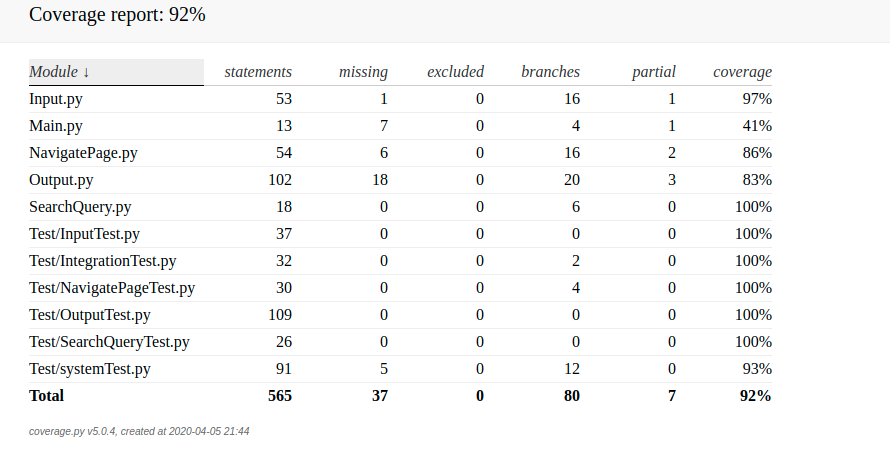
\includegraphics[scale=0.5]{branch.png}
    \caption{Branch Coverage Results}
    \label{fig:Branch Coverage}
\end{figure}

\begin{figure}[htp]
    \centering
    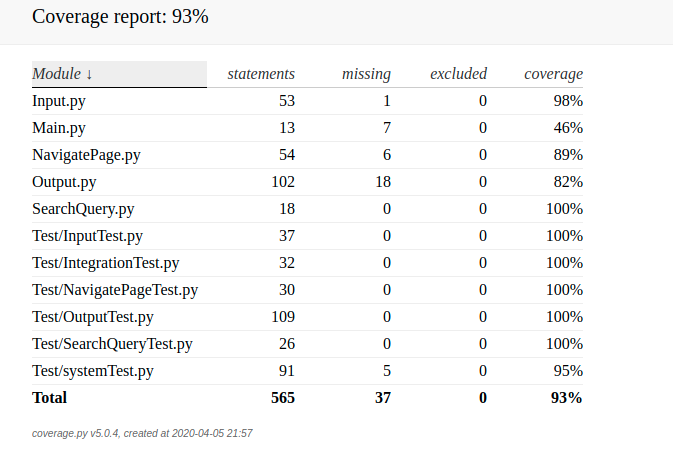
\includegraphics[scale=0.5]{statement-coverage.png}
    \caption{Statement Coverage Results}
    \label{fig:Statement Coverage}
\end{figure}

\bibliographystyle{plainnat}

\bibliography{SRS}

\end{document}